% This file was created by tikzplotlib v0.9.8.
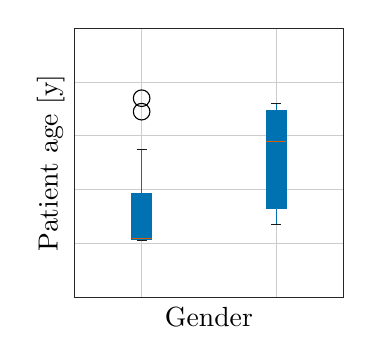
\begin{tikzpicture}

\definecolor{color0}{rgb}{0,0.447058823529412,0.698039215686274}
\definecolor{color1}{rgb}{0.835294117647059,0.368627450980392,0}

\begin{axis}[
axis line style={white!15!black},
height=5cm,
tick align=outside,
width=5cm,
x grid style={white!80!black},
xlabel={Gender},
xmajorgrids,
xmajorticks=false,
xmin=0.5, xmax=2.5,
xtick style={color=white!15!black},
xtick={1,2},
xticklabels={F(11),M(6)},
y grid style={white!80!black},
ylabel={Patient age [y]},
ymajorgrids,
ymajorticks=false,
ymin=0, ymax=100,
ytick style={color=white!15!black}
]
\addplot [color0, opacity=1]
table {%
1 21.5
1 21
};
\addplot [color0, opacity=1]
table {%
1 38.5
1 55
};
\addplot [white!10!black, opacity=1]
table {%
0.9625 21
1.0375 21
};
\addplot [white!10!black, opacity=1]
table {%
0.9625 55
1.0375 55
};
\addplot [black, mark=o, mark size=3, mark options={solid,fill opacity=0}, only marks]
table {%
1 74
1 69
};
\addplot [color0, opacity=1]
table {%
2 33
2 27
};
\addplot [color0, opacity=1]
table {%
2 69.5
2 72
};
\addplot [white!10!black, opacity=1]
table {%
1.9625 27
2.0375 27
};
\addplot [white!10!black, opacity=1]
table {%
1.9625 72
2.0375 72
};
\path [draw=color0, fill=color0]
(axis cs:0.925,21.5)
--(axis cs:1.075,21.5)
--(axis cs:1.075,38.5)
--(axis cs:0.925,38.5)
--(axis cs:0.925,21.5)
--cycle;
\path [draw=color0, fill=color0]
(axis cs:1.925,33)
--(axis cs:2.075,33)
--(axis cs:2.075,69.5)
--(axis cs:1.925,69.5)
--(axis cs:1.925,33)
--cycle;
\addplot [color1, opacity=1]
table {%
0.925 22
1.075 22
};
\addplot [color1, opacity=1]
table {%
1.925 58
2.075 58
};
\end{axis}

\end{tikzpicture}
